%!TEX root = ./main.tex

%%**************************************************************
%%
%% DHBW Heidenheim - Template for Bachelor Thesis
%%
%% For further information see REAMDME.md
%%
%%**************************************************************

%!TEX root = ../main.tex

% show warning for old LaTeX syntax
\RequirePackage[l2tabu, orthodox]{nag}

\documentclass[
	pdftex,
	oneside,  
	12pt,			    % fontsize
	parskip=half,		    % Space (in lines) between paragraphs
	headheight = 12pt,    % Header hight
	headsepline,		    % Line after header
	footheight = 16pt,	    % Footer height
	footsepline,		    % Line before footer
	abstracton,		    % Abstract headline
	DIV=calc,		    % Calculate print space
	BCOR=8mm,		    % BCOR settings (Bindekorrektur)
	headinclude=false,   % Exclude header from print space
	footinclude=false,	    % Exclude footer from print space
	listof=totoc,		    % Show List of Figures/Tables in Contents
	toc=bibliography,	    % Show Bibliography in Contents
]{scrreprt}	                     % Koma-Script report-class, long document: scrreprt, short document: scrbook

\usepackage{xstring}
\usepackage[utf8]{inputenc}
\usepackage[T1]{fontenc}

% iflang command definition
\newcommand{\iflang}[2]{%
  \IfStrEq{\documentLanguage}{#1}{#2}{}
}

% ifDocType comand definition
\newcommand{\ifDocType}[2]{%
  \IfStrEq{\documentType}{#1}{#2}{}
}

% Include main settings
%!TEX root = ../main.tex

%% Citation Styles
% http://ctan.mirrorcatalogs.com/macros/latex/contrib/biblatex/doc/biblatex.pdf (3.3.1 Citation Styles)
% recommended:  z.B numeric-comp, alphabetic, 
% not recommended: authoryear, alphabetic-verb, 
\newcommand{\quoteStyle}{numeric-comp}

%% Fonts
%% palatino, goudysans, lmodern or libertine
\newcommand{\documentFont}{lmodern}

%% Margin
\newcommand{\margin}{2.5cm}

%% Space between chapter headline and top of page
\newcommand{\chapterMargin}{20pt}

%% Table settings
% Column spacing
\newcommand{\tableColumnMargin}{10pt}
%Line spacing
\newcommand{\tableRowMargin}{1.5}

%% Color settings
\newcommand{\defineColors}{%
	\definecolor{LinkColor}{HTML}{00007A}
	\definecolor{ListingBackground}{HTML}{ebf7ec}
}

%% Syntax Highlighting (Listings)
\newcommand{\listingsettings}{%
	\lstset{%
		language=Java,			% default language
		numbers=left,			% position of line numbers (left, right)
		stepnumber=1,			% set number to each line
		numbersep=5pt,			% 5pt between number and source code
		numberstyle=\tiny,		% letter size of numbers
		breaklines=true,		        % break lines if necessary (true, false)
		breakautoindent=true,	        % indenting after break line (true, false)
		postbreak=\space,		% break line after space
		tabsize=2,				% tabulator size
		basicstyle=\ttfamily\footnotesize, % font style
		showspaces=false,		% show space (true, false)		showstringspaces=false,	% show space in strings (true, false)
		extendedchars=true,		% show all Latin1 characters (true, false)
		captionpos=b,			% sets the caption-position to bottom
		backgroundcolor=\color{ListingBackground}, % source code background
		xleftmargin=0pt,		        % margin left
		xrightmargin=0pt,		        % margin right
		frame=single,			        % border settings
		frameround=ffff,
		rulecolor=\color{darkgray},	% border color
		fillcolor=\color{ListingBackground},
		keywordstyle=\color[rgb]{0.133,0.133,0.6},
		commentstyle=\color[rgb]{0.133,0.545,0.133},
		stringstyle=\color[rgb]{0.627,0.126,0.941}
	}
}
 

% Include document settings
%!TEX root = ../main.tex

%% Document language (en, de)
\newcommand{\documentLanguage}{en}

%% Document type
% T2\_1000 Project Thesis (Semester 1 & 2)
% T2\_2000 Project Thesis (Semester 3 & 4)
% T2\_3100 Seminar Paper (Semester 5 & 6)
% T2\_3300 Bachelor Thesis
\newcommand{\documentType}{T2\_3300}

\newcommand{\documentAuthor}{Lisa Boos, Sergej Dechant, Khaled Jallouli, Martin Schmid}
\newcommand{\documentTitle}{Predicting the Outcome of Soccer Matches}
\newcommand{\documentPeriod}{6 months}

\newcommand{\matriculationNumber}{3133068}

\newcommand{\locationUniversity}{Ulm}
\newcommand{\department}{Informationssysteme}
\newcommand{\course}{}

\newcommand{\degree}{Master of Science}
% INF2014 - INF2016 (MI):         Bachelor of Science
% INF2014 - INF2016 (IA/IM) :   Bachelor of Engineering
% INF2017 (all):                             Bachelor of Science

\newcommand{\releaseDate}{February 2020}
\newcommand{\releaseLocation}{Ulm}

%\newcommand{\companyName}{ZwickRoell GmbH \& Co.KG}
%\newcommand{\companyLocation}{Ulm/Einsingen}

\newcommand{\tutor}{Prof. Dr. Goldstein}
\newcommand{\evaluator}{Prof. Dr. Herbort}

% Load language specific Strings
\input{lang/\documentLanguage}

% Load language specific babel package
\iflang{de}{\usepackage[english, ngerman]{babel}}
\iflang{en}{\usepackage[ngerman, english]{babel}} 

% Add comment feature
\newcommand{\comment}[1]{\par {\bfseries \color{blue} #1 \par}}


%%%%%%% Package Includes %%%%%%%

\usepackage[margin=\margin,foot=1cm]{geometry}
\usepackage[activate]{microtype}                                         
\usepackage[onehalfspacing]{setspace}
\usepackage{makeidx}
\usepackage[autostyle=true,german=quotes]{csquotes}
\usepackage{longtable}
\usepackage{enumitem}	                                                 
\usepackage{graphicx}
\usepackage{pdfpages}                                                         
\usepackage{xcolor} 	                                                    
\usepackage{float}
\usepackage{array}
\usepackage{calc}		                         
\usepackage[right]{eurosym}
\usepackage{wrapfig}
\usepackage{pgffor}                                                             
\usepackage[perpage, hang, multiple, stable]{footmisc}  
\usepackage[printonlyused]{acronym}                                 
\usepackage{listings}
\usepackage[obeyFinal,backgroundcolor=yellow,linecolor=black]{todonotes}
\usepackage{rotating}
\usepackage{lscape}
\usepackage{amsmath}
\usepackage{amssymb}
\usepackage{\documentFont}
\usepackage[%
	pdftitle={\documentTitle},
	pdfauthor={\documentAuthor},
	pdfsubject={\documentType},
	pdfcreator={pdflatex, LaTeX with KOMA-Script},
	pdfpagemode=UseOutlines,       % Show Contents while opening
	pdfdisplaydoctitle=true, 		% Show document title instead of file name
	pdflang={\documentLanguage}, % Document language
]{hyperref}
\usepackage{bookmark}
\usepackage[nonumberlist,toc]{glossaries}

% Load colors
\defineColors{}

% Set Titel, Autor and Date
\title{\documentTitle}
\author{\documentAuthor}
\date{\datum}


% PDF link settings
\hypersetup{%
	colorlinks=true, 		
	linkcolor=LinkColor, 	
	citecolor=LinkColor,
	filecolor=LinkColor,
	menucolor=LinkColor,
	urlcolor=LinkColor,
	linktocpage=true, 
	bookmarksnumbered=true 
}

% Captions fontsize
\addtokomafont{caption}{\small}

% Bibliographie settings
\iflang{de}{%
\usepackage[
	backend=biber,		% recommended. Alternative: bibtex
	bibwarn=true,
	bibencoding=utf8,	         % If .bib file is encoded with utf8, otherwise ascii
	sortlocale=de_DE,
	style=\quoteStyle,
]{biblatex}
}
\iflang{en}{%
\usepackage[
	backend=biber,		% recommended. Alternative: bibtex
	bibwarn=true,
	bibencoding=utf8,        % If .bib file is encoded with utf8, otherwise ascii
	sortlocale=en_US,
	style=\quoteStyle,
]{biblatex}
}

\addbibresource{bibliographie.bib}

% Hurenkinder und Schusterjungen verhindern
% http://projekte.dante.de/DanteFAQ/Silbentrennung
\clubpenalty = 10000 % schließt Schusterjungen aus (Seitenumbruch nach der ersten Zeile eines neuen Absatzes)
\widowpenalty = 10000 % schließt Hurenkinder aus (die letzte Zeile eines Absatzes steht auf einer neuen Seite)
\displaywidowpenalty=10000

% Graphicspath
\graphicspath{{images/}}

% frequently used programing languages
\lstloadlanguages{PHP,Python,Java,C,C++,bash}

\listingsettings{}
% Rename Listings
\renewcommand\lstlistingname{\listingPhrase}
\renewcommand\lstlistlistingname{\listListingPhrase}
\def\lstlistingautorefname{\authorListingPhrase}

% Spaces in tables
\setlength{\tabcolsep}{\tableColumnMargin}
\renewcommand{\arraystretch}{\tableRowMargin}


%!TEX root = ../main.tex

%
% To create glossary run the following command: 
% makeglossaries main.acn && makeglossaries main.glo
%

%
% Glossareintraege --> referenz, name, beschreibung
% Aufruf mit \gls{...}
%
\newglossaryentry{Glossareintrag}{name={Glossareintrag},plural={Glossareinträge},description={Ein Glossar beschreibt verschiedenste Dinge in kurzen Worten}}


\begin{document}

	% Cover
	\begin{spacing}{1}
		%!TEX root = ../main.tex

\begin{titlepage}
	\begin{longtable}{p{8cm} p{8cm}}
		\raggedright {\raisebox{\ht\strutbox-\totalheight}{
\includegraphics[height=2.5cm]{images/HS.png}}} &
		%\raggedleft {\raisebox{\ht\strutbox-\totalheight}{\includegraphics[height=2cm]{images/cover/HSULM.jfif}}}
	\end{longtable}
	\enlargethispage{20mm}
	\begin{center}
    \doublespacing{
		\vspace*{12mm}	{\LARGE\textbf \documentTitle }}\\
		%\vspace*{12mm}	{\large\textbf housework}\\
		\vspace*{12mm}	\degreePhrase\\
		\vspace*{3mm}		{\textbf \degree}\\
		\vspace*{12mm}	\departmentPhrase{} \department\\
    \vspace*{0mm}		at the Technische Hochschule in Ulm \\
		\vspace*{12mm}	\documentAuthorPhrase\\
		\vspace*{3mm}		{\large\textbf \documentAuthor}\\
		\vspace*{12mm}	\releaseDate\\
	\end{center}
	\vfill
	\begin{spacing}{1.2}
	\begin{tabbing}
		mmmmmmmmmmmmmmmmmmmmmmmmmm             \= \kill
	%	\textbf{\documentPeriodPhrase}       \>  \documentPeriod\\
		%\textbf{\matriculationNumberPhrase}  \>  \matriculationNumber\\
	%	\textbf{\companyPhrase}                  \>  \companyName, \companyLocation\\
		\textbf{\tutorPhrase}               \>  \tutor\\
		\textbf{\evaluatorPhrase}              \>  \evaluator
	\end{tabbing}
	\end{spacing}
\end{titlepage}

	\end{spacing}
	\newpage

	\pagenumbering{Roman}

	% Restriction notices
	%%!TEX root = ../main.tex

\thispagestyle{empty}

\section*{\restrictionNoticesPhrase}

\vspace*{2em}

\iflang{de}{%
  Die vorliegende {\documentTypePhrase} mit dem Titel {\itshape{} \documentTitle{}\/} enthält 
  unternehmensinterne bzw. vertrauliche Informationen der {\companyName}, ist deshalb mit einem 
  Sperrvermerk versehen und wird ausschließlich zu Prüfungszwecken am Studiengang {\department} 
  der Dualen Hochschule Baden-Württemberg {\locationUniversity} vorgelegt. Sie ist ausschließlich zur 
  Einsicht durch den zugeteilten Gutachter, die Leitung des Studiengangs und ggf. den Prüfungsausschuss 
  des Studiengangs bestimmt.  Es ist untersagt,
  \begin{itemize}
  \item den Inhalt dieser Arbeit (einschließlich Daten, Abbildungen, Tabellen, Zeichnungen usw.) als 
            Ganzes oder auszugsweise weiterzugeben,
  \item Kopien oder Abschriften dieser Arbeit (einschließlich Daten, Abbildungen, Tabellen, 
             Zeichnungen usw.) als Ganzes oder in Auszügen anzufertigen,
  \item diese Arbeit zu veröffentlichen bzw. digital, elektronisch oder virtuell zur Verfügung zu stellen. 
  \end{itemize}
Jede anderweitige Einsichtnahme und Veröffentlichung – auch von Teilen der Arbeit – bedarf der 
vorherigen Zustimmung durch den Verfasser und {\companyName}.
}

%http://www.ib.dhbw-mannheim.de/fileadmin/ms/bwl-ib/Downloads_alt/Leitfaden_31.05.pdf

\iflang{en}{%
  The {\documentTypePhrase} on hand
  \begin{center}{\itshape{} \documentTitle{}\/}\end{center}
   contains internal resp.\ confidential data of {\companyName}. It is intended solely for inspection by the
   assigned examiner, the head of the {\department} department and, if necessary, the Audit
   Committee \locationUniversityPhrase{} {\locationUniversity}. It is strictly forbidden
    \begin{itemize}
    \item to distribute the content of this paper (including data, figures, tables, charts etc.) as a whole or 
              in extracts,
    \item to make copies or transcripts of this paper or of parts of it,
    \item to display this paper or make it available in digital, electronic or virtual form.
    \end{itemize}
  Exceptional cases may be considered through permission granted in written form by the author 
  and {\companyName}.
}

\vspace{3em}

\releaseLocation, \releaseDate
\vspace{4em}

\rule{6cm}{0.4pt}\\
\documentAuthor

	%\newpage

	% Declaration
	%!TEX root = ../main.tex

\thispagestyle{empty}

\section*{\declarationPhrase}

\vspace*{2em}

\iflang{de}{%
  Ich versichere hiermit, dass ich die vorliegende Arbeit mit dem Thema: {\itshape \documentTitle } 
  selbstständig verfasst und  keine anderen als die angegebenen Quellen und Hilfsmittel benutzt habe. 
  Ich versichere zudem, dass die eingereichte elektronische Fassung mit der gedruckten Fassung 
  übereinstimmt. 
}


\iflang{en}{%
  Hereby I solemnly declare:
  \begin{enumerate}
  \item that this document, titled {\itshape \documentTitle } is entirely the product of my 
            own scholarly work, unless otherwise indicated in the text or references, or acknowledged below;
  \item I have indicated the thoughts adopted directly or indirectly from other sources at the appropriate 
            places within the document;
  \item this document has not been submitted either in whole or part, for a degree at this or 
            any other university or institution;
  \item I have not published this document in the past.
  \end{enumerate}
  I am aware that a dishonest declaration will entail legal consequences.
}

\vspace{3em}

\releaseLocation, \releaseDate
\vspace{4em}

\rule{6cm}{0.4pt}\\
\documentAuthor

	\newpage

	% Abstract
	%!TEX root = ../main.tex

\pagestyle{empty}

% override abstract headline

%\renewcommand{\abstractname}{Zusammenfassung}
%
%\begin{abstract}
%
%lorem ipsum
%
%\end{abstract}

\renewcommand{\abstractname}{Abstract}

\begin{abstract}

lorem ipsum


\end{abstract}
	\newpage

        % only page number in footer
	\pagestyle{plain}
	
	% space bevore chapter headline
	\RedeclareSectionCommand[beforeskip=\chapterMargin]{chapter}

	% Contents
	\begin{spacing}{1.1}
		\begingroup
		
		        % set subchapter depth
			\setcounter{tocdepth}{1}
			
			\tableofcontents
			\clearpage
		\endgroup
	\end{spacing}
	\newpage

	% Acronyms
	\cleardoublepage
        %!TEX root = ../main.tex

\addchap{\acronymsPhrase}

\begin{acronym}[YTMMM]
\setlength{\itemsep}{-\parsep}

\acro{UR}{Universal Robots Leichtbau Roboter}
\acro{IPC}{Industrie PC}
\acro{ST}{Structured Text}
\acro{E/As}{Eingänge/Ausgänge}
\acro{FB}{Funktionsbaustein}
\acro{FC}{Funktion (Function)}
\acro{SPS}{Speicherprogrammierbare Steuerung}
\acro{SoftSPS}{Software, die eine Speicherprogrammierbare Steuerung bereit stellt}
\acro{PTP}{Punkt zu Punkt Fahrt (Point  to Point)} 
\acro{Hasy}{Automatisiertes Mehrachssystem (Handling System) } 
\acro{SCL}{Structured Control Language}
\end{acronym}


	% List of Figures
	\cleardoublepage
	\listoffigures

	%List of Tables
	\cleardoublepage
	\listoftables

	% List of Listings
	\cleardoublepage
	\lstlistoflistings
	\cleardoublepage

	\pagenumbering{arabic}
	
	\pagestyle{headings}

	%Content
	\foreach \i in {01,02,03,04,05,06,07,08,09,...,99} {%
		\edef\FileName{content/chapter/\i .tex}%
			\IfFileExists{\FileName}{%
				\input{\FileName}
			}
			{%
%				No chapter available
			}
}

	\clearpage

	% Bibilography
	\cleardoublepage
	\printbibliography

	% Glossar
	\printglossary[style=altlist,title=\glossaryPhrase]
	
	% Appendix
	\clearpage
	\appendix
	% !TeX root = ../main.tex

\chapter{Appendix}
\section{Architectures for various neural nets}
\label{section:appendix_a}
\begin{longtable}{|l|l|l|l|l|l|l|}
\caption{Test Variation of Hidden-Layers and Neurons for Neural Nets} \\
\hline
\textbf{Name} & \textbf{Input} & \textbf{HLayer1} & \textbf{HLayer2} & \textbf{HLayer3} & \textbf{HLayer4} & \textbf{Output} \\ 
\hline
\endfirsthead
\hline
\textbf{Name} & \textbf{Input} & \textbf{HLayer1} & \textbf{HLayer2} & \textbf{HLayer3} & \textbf{HLayer4} & \textbf{Output} \\ 
\hline
\endhead
\multicolumn{7}{r}{continued on next page}\\
\endfoot
\hline
\multicolumn{7}{r}{end of table} \\
\endlastfoot
model01\_H1\_H & 13 & 13 & - & - & - & 3 \\ \hline
model02\_H1\_H & 21 & 21 & - & - & - & 3 \\ \hline
model03\_H1\_H & 29 & 29 & - & - & - & 3 \\ \hline
model04\_H1\_H & 25 & 25 & - & - & - & 3 \\ \hline
model05\_H1\_H & 33 & 33 & - & - & - & 3 \\ \hline
model01\_H1\_M & 13 & 9 & - & - & - & 3 \\ \hline
model02\_H1\_M & 21 & 12 & - & - & - & 3 \\ \hline
model03\_H1\_M & 29 & 14 & - & - & - & 3 \\ \hline
model04\_H1\_M & 25 & 13 & - & - & - & 3 \\ \hline
model05\_H1\_M & 33 & 16 & - & - & - & 3 \\ \hline
model01\_H1\_L & 13 & 4 & - & - & - & 3 \\ \hline
model02\_H1\_L & 21 & 5 & - & - & - & 3 \\ \hline
model03\_H1\_L & 29 & 7 & - & - & - & 3 \\ \hline
model04\_H1\_L & 25 & 6 & - & - & - & 3 \\ \hline
model05\_H1\_L & 33 & 8 & - & - & - & 3 \\ \hline
model01\_H2\_H & 13 & 13 & 13 & - & - & 3 \\ \hline
model02\_H2\_H & 21 & 21 & 21 & - & - & 3 \\ \hline
model03\_H2\_H & 29 & 29 & 29 & - & - & 3 \\ \hline
model04\_H2\_H & 25 & 25 & 25 & - & - & 3 \\ \hline
model05\_H2\_H & 33 & 33 & 33 & - & - & 3 \\ \hline
model01\_H2\_M & 13 & 9 & 9 & - & - & 3 \\ \hline
model02\_H2\_M & 21 & 12 & 12 & - & - & 3 \\ \hline
model03\_H2\_M & 29 & 14 & 14 & - & - & 3 \\ \hline
model04\_H2\_M & 25 & 13 & 13 & - & - & 3 \\ \hline
model05\_H2\_M & 33 & 16 & 16 & - & - & 3 \\ \hline
model01\_H2\_L & 13 & 4 & 4 & - & - & 3 \\ \hline
model02\_H2\_L & 21 & 5 & 5 & - & - & 3 \\ \hline
model03\_H2\_L & 29 & 7 & 7 & - & - & 3 \\ \hline
model04\_H2\_L & 25 & 6 & 6 & - & - & 3 \\ \hline
model05\_H2\_L & 33 & 8 & 8 & - & - & 3 \\ \hline
model01\_H3\_H & 13 & 13 & 13 & 13 & - & 3 \\ \hline
model02\_H3\_H & 21 & 21 & 21 & 21 & - & 3 \\ \hline
model03\_H3\_H & 29 & 29 & 29 & 29 & - & 3 \\ \hline
model04\_H3\_H & 25 & 25 & 25 & 25 & - & 3 \\ \hline
model05\_H3\_H & 33 & 33 & 33 & 33 & - & 3 \\ \hline
model01\_H3\_M & 13 & 9 & 9 & 9 & - & 3 \\ \hline
model02\_H3\_M & 21 & 12 & 12 & 12 & - & 3 \\ \hline
model03\_H3\_M & 29 & 14 & 14 & 14 & - & 3 \\ \hline
model04\_H3\_M & 25 & 13 & 13 & 13 & - & 3 \\ \hline
model05\_H3\_M & 33 & 16 & 16 & 16 & - & 3 \\ \hline
model01\_H3\_L & 13 & 4 & 4 & 4 & - & 3 \\ \hline
model02\_H3\_L & 21 & 5 & 5 & 5 & - & 3 \\ \hline
model03\_H3\_L & 29 & 7 & 7 & 7 & - & 3 \\ \hline
model04\_H3\_L & 25 & 6 & 6 & 6 & - & 3 \\ \hline
model05\_H3\_L & 33 & 8 & 8 & 8 & - & 3 \\ \hline
model01\_H3\_F & 13 & 13 & 10 & 7 & 5 & 3 \\ \hline
model02\_H3\_F & 21 & 18 & 13 & 9 & 5 & 3 \\ \hline
model03\_H3\_F & 29 & 22 & 16 & 11 & 6 & 3 \\ \hline
model04\_H3\_F & 25 & 20 & 15 & 11 & 6 & 3 \\ \hline
model05\_H3\_F & 33 & 25 & 19 & 12 & 6 & 3 \\ \hline
model01\_H4\_H & 13 & 13 & 13 & 13 & 13 & 3 \\ \hline
model02\_H4\_H & 21 & 21 & 21 & 21 & 21 & 3 \\ \hline
model03\_H4\_H & 29 & 29 & 29 & 29 & 29 & 3 \\ \hline
model04\_H4\_H & 25 & 25 & 25 & 25 & 25 & 3 \\ \hline
model05\_H4\_H & 33 & 33 & 33 & 33 & 33 & 3 \\ \hline
model01\_H4\_M & 13 & 9 & 9 & 9 & 9 & 3 \\ \hline
model02\_H4\_M & 21 & 12 & 12 & 12 & 12 & 3 \\ \hline
model03\_H4\_M & 29 & 14 & 14 & 14 & 14 & 3 \\ \hline
model04\_H4\_M & 25 & 13 & 13 & 13 & 13 & 3 \\ \hline
model05\_H4\_M & 33 & 16 & 16 & 16 & 16 & 3 \\ \hline
model01\_H4\_L & 13 & 4 & 4 & 4 & 4 & 3 \\ \hline
model02\_H4\_L & 21 & 5 & 5 & 5 & 5 & 3 \\ \hline
model03\_H4\_L & 29 & 7 & 7 & 7 & 7 & 3 \\ \hline
model04\_H4\_L & 25 & 6 & 6 & 6 & 6 & 3 \\ \hline
model05\_H4\_L & 33 & 8 & 8 & 8 & 8 & 3 \\ \hline
model01\_H4\_F & 13 & 13 & 10 & 7 & 5 & 3 \\ \hline
model02\_H4\_F & 21 & 18 & 13 & 9 & 5 & 3 \\ \hline
model03\_H4\_F & 29 & 22 & 16 & 11 & 6 & 3 \\ \hline
model04\_H4\_F & 25 & 20 & 15 & 11 & 6 & 3 \\ \hline
model05\_H4\_F & 33 & 25 & 19 & 12 & 6 & 3 \\ \hline
\end{longtable}

\newpage
\section{Daily Scrum Logs}
\label{section:appendix_b}
TODO: insert daily scrum logs
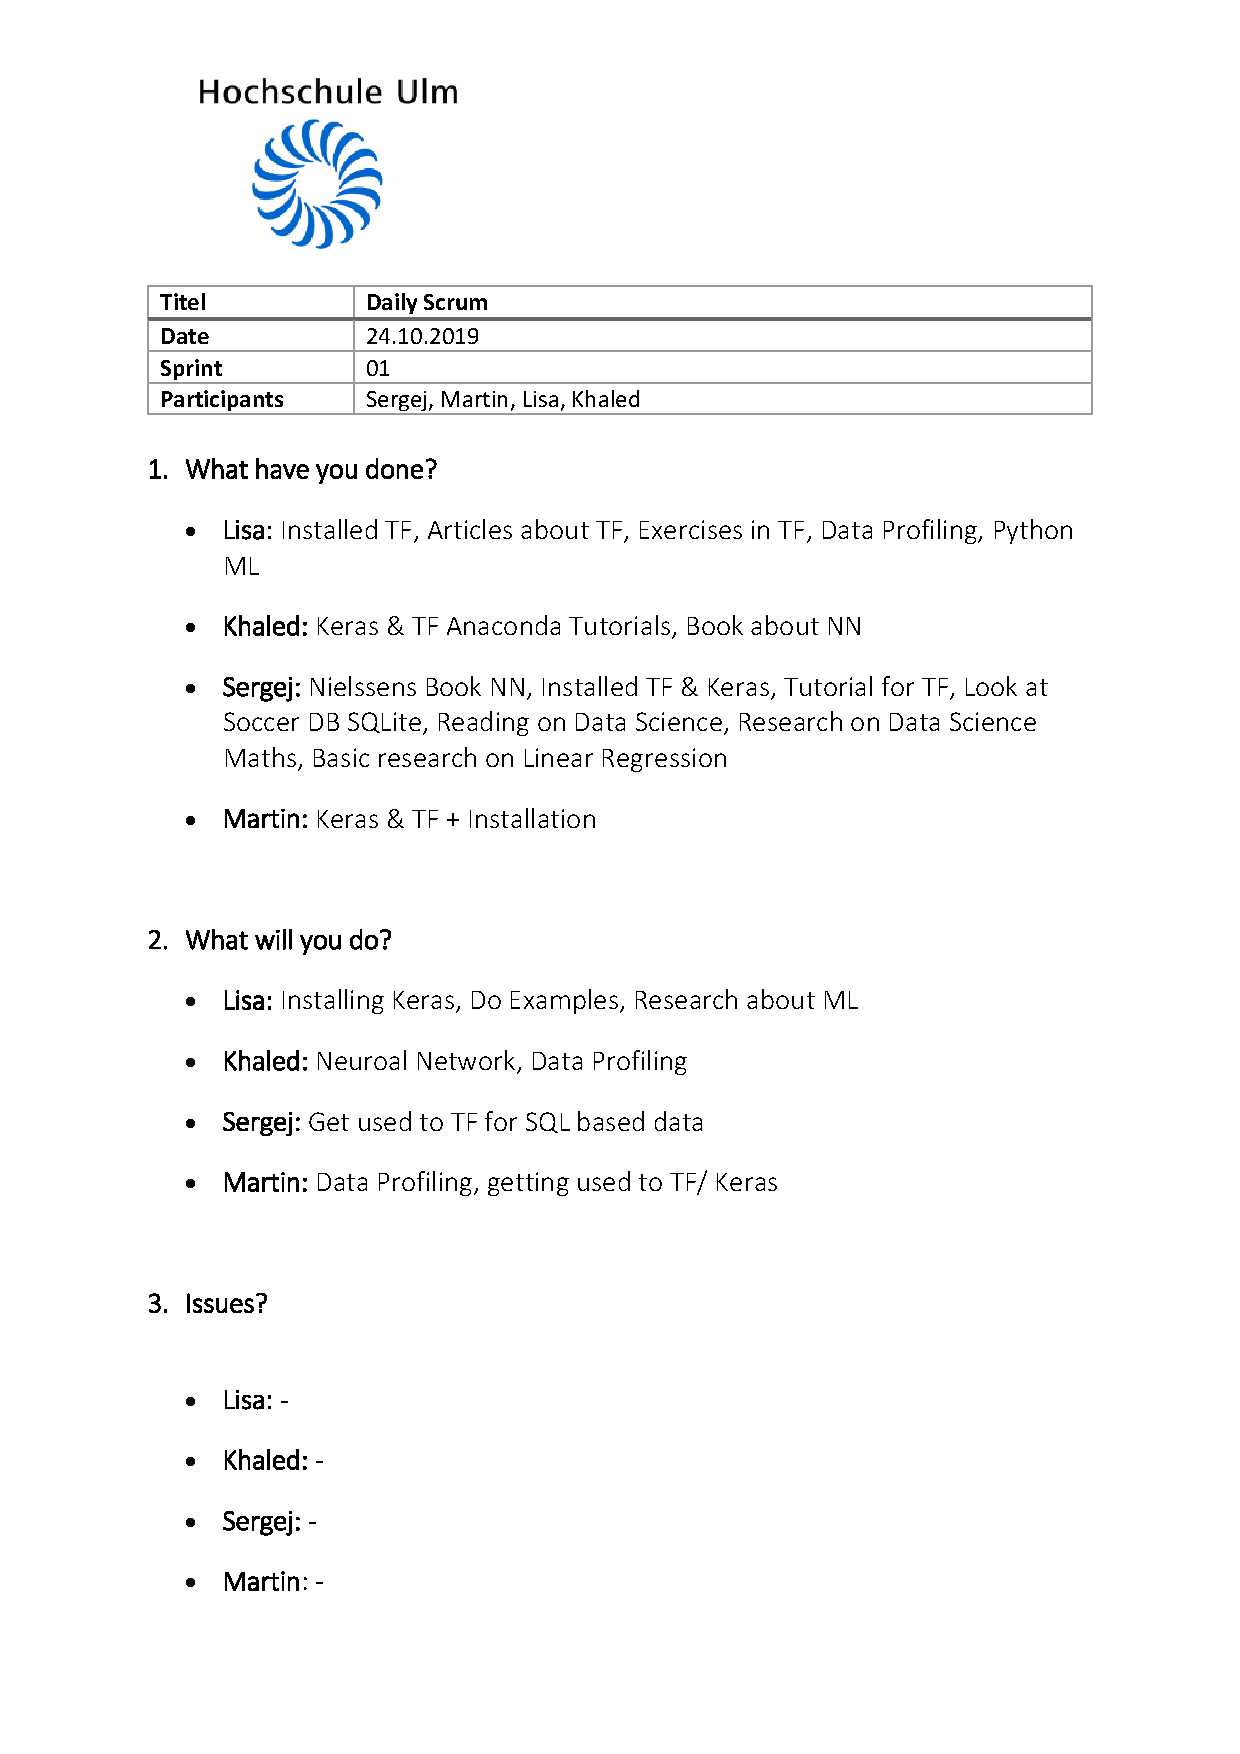
\includepdf[pages={1-2}]{pdf/Daily_Scrum_S01_1.pdf}
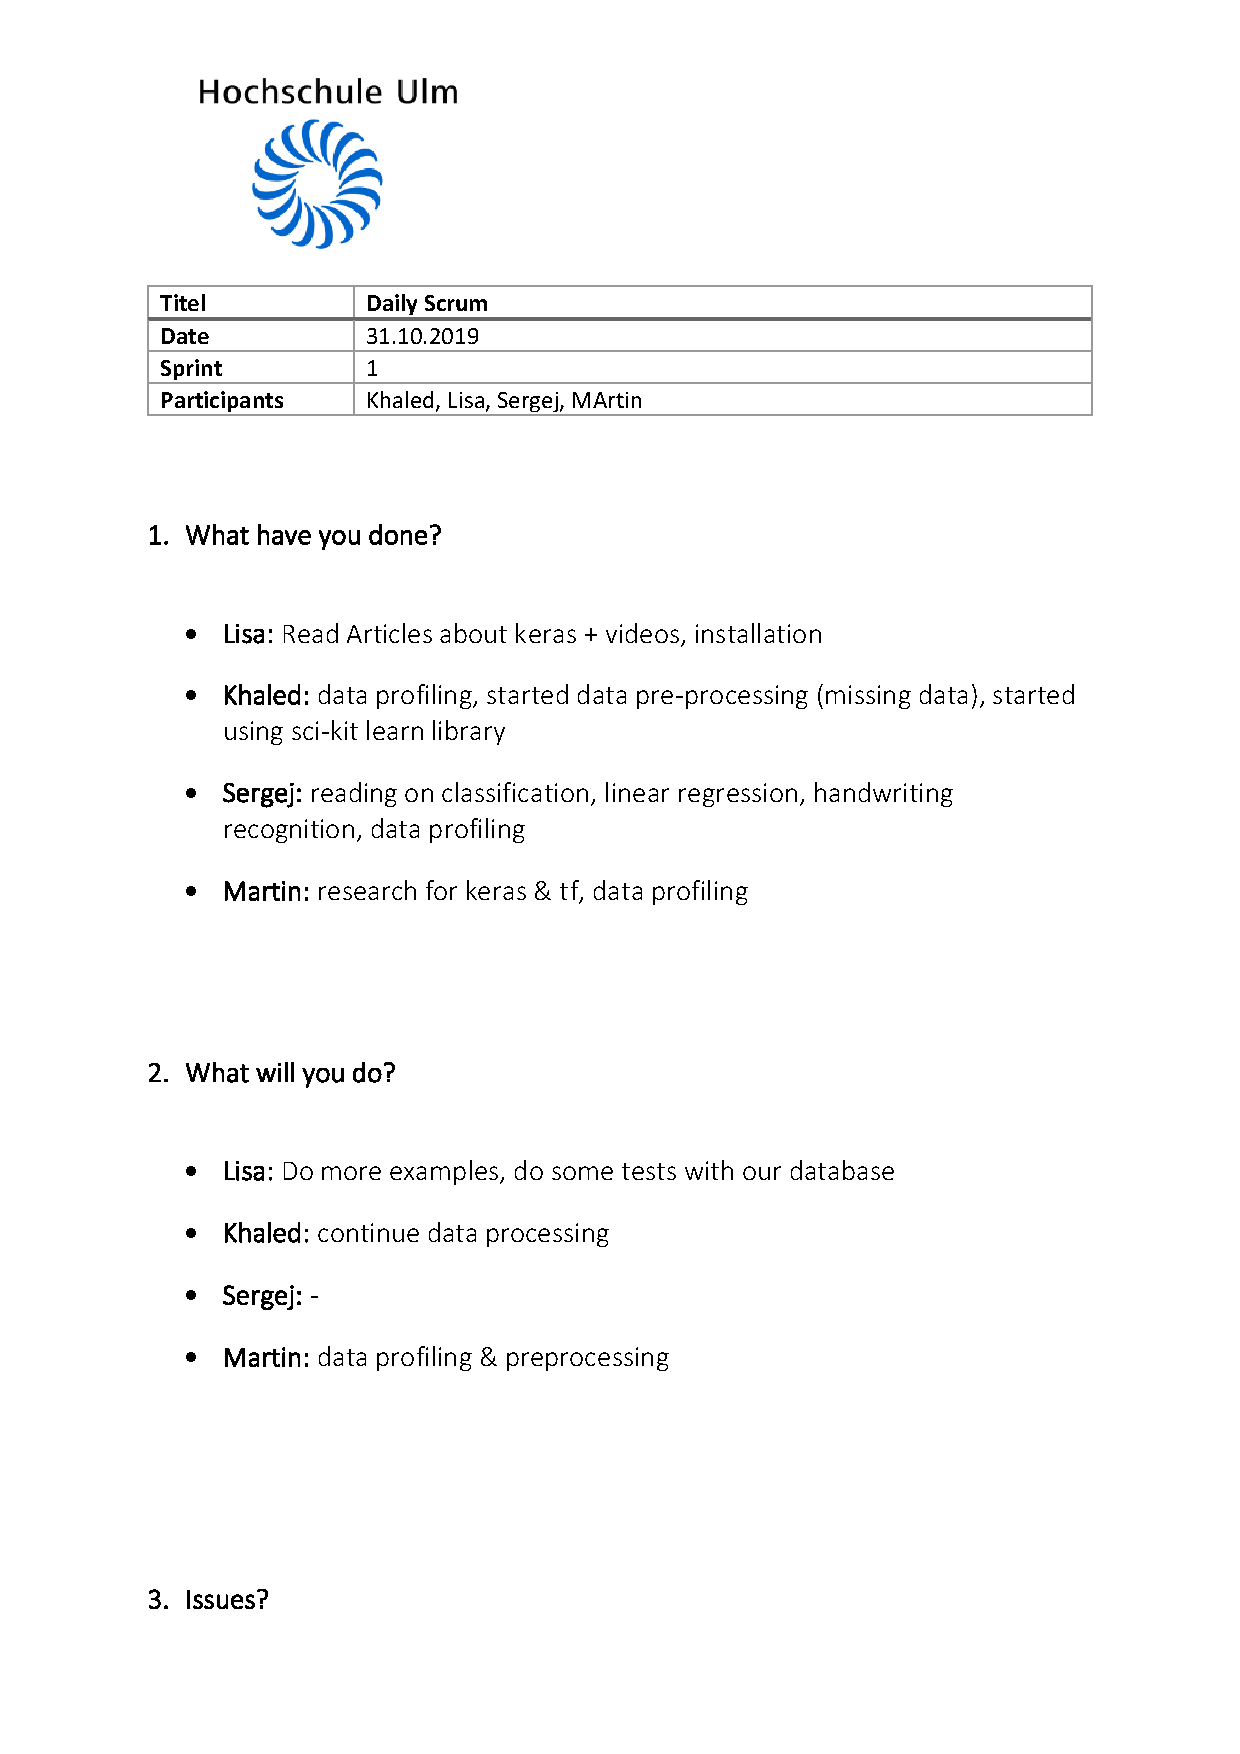
\includepdf[pages={1-2}]{pdf/Daily_Scrum_S01_2.pdf}
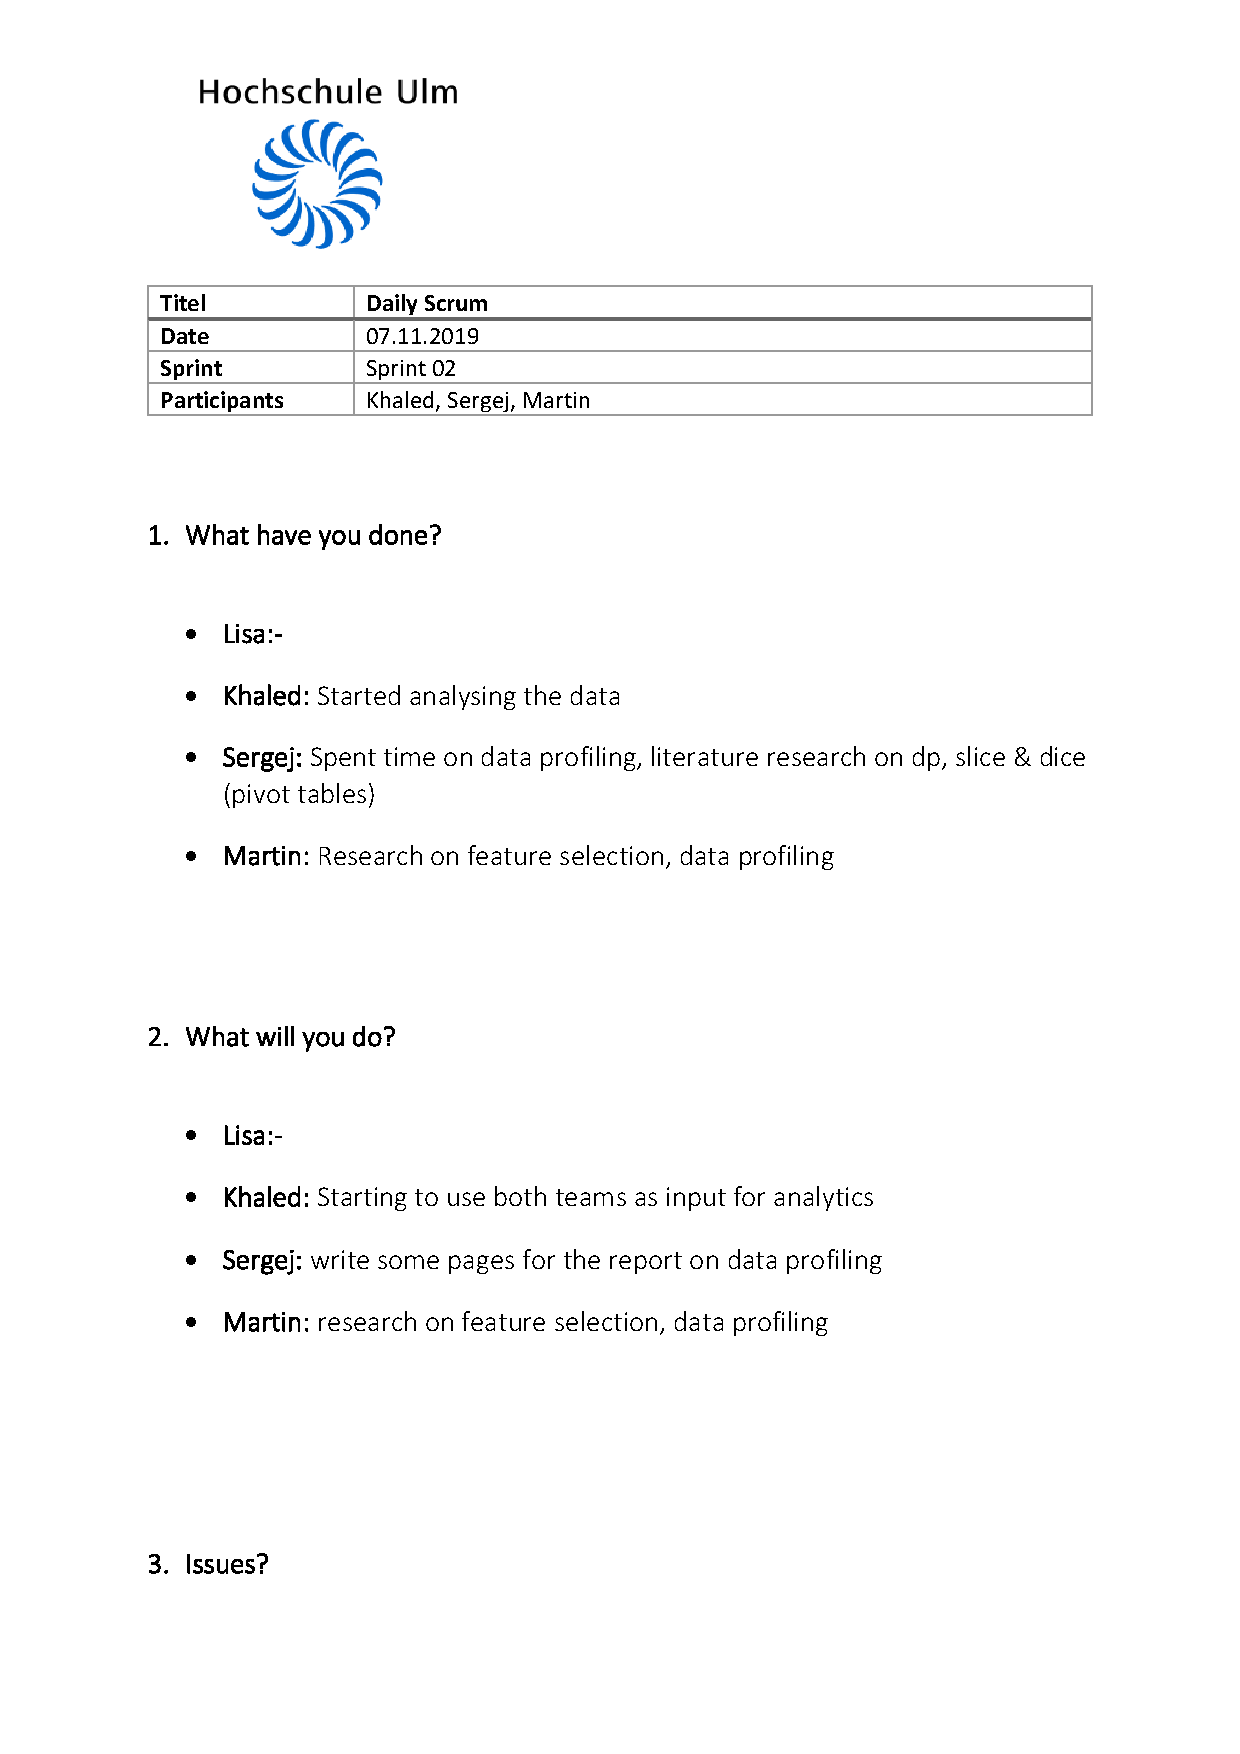
\includepdf[pages={1-2}]{pdf/Daily_Scrum_S02_1.pdf}
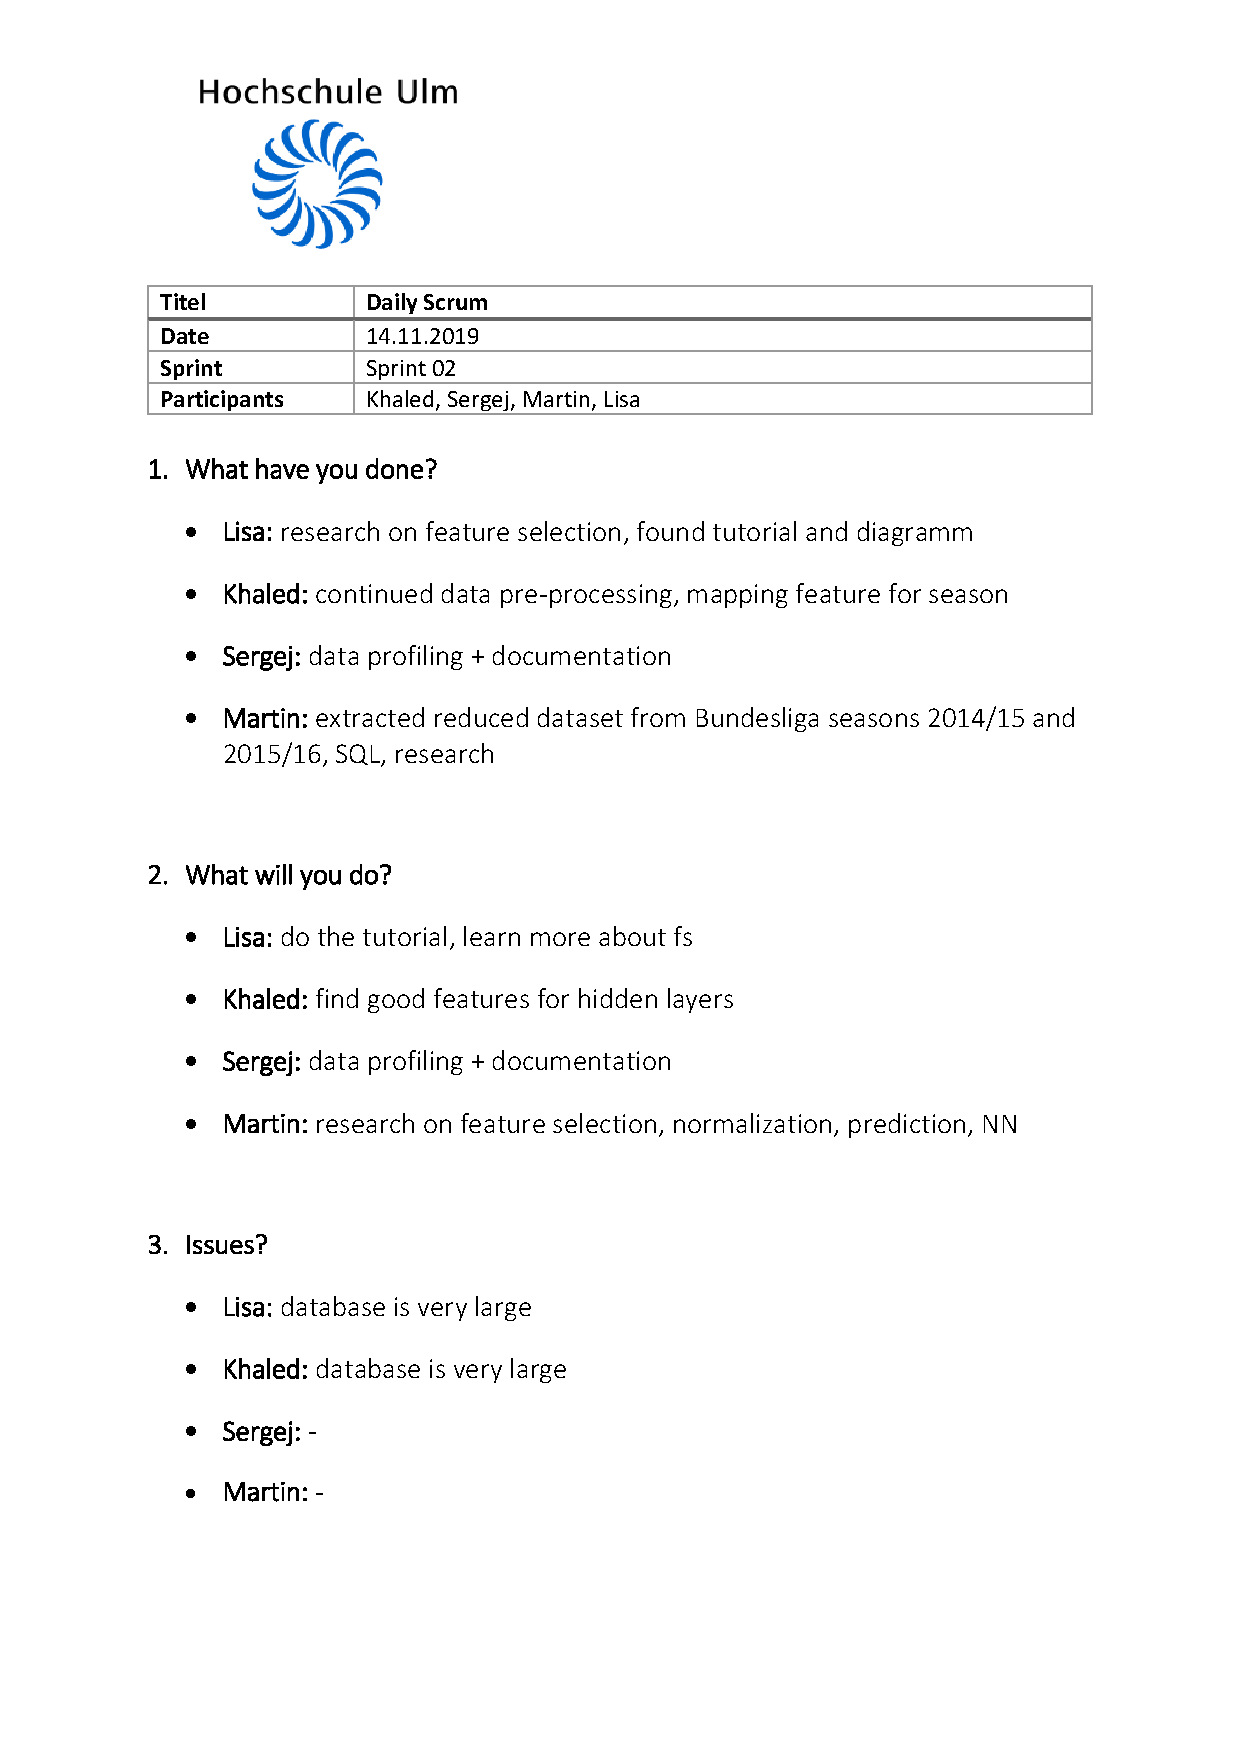
\includepdf[pages={1-2}]{pdf/Daily_Scrum_S02_2.pdf}
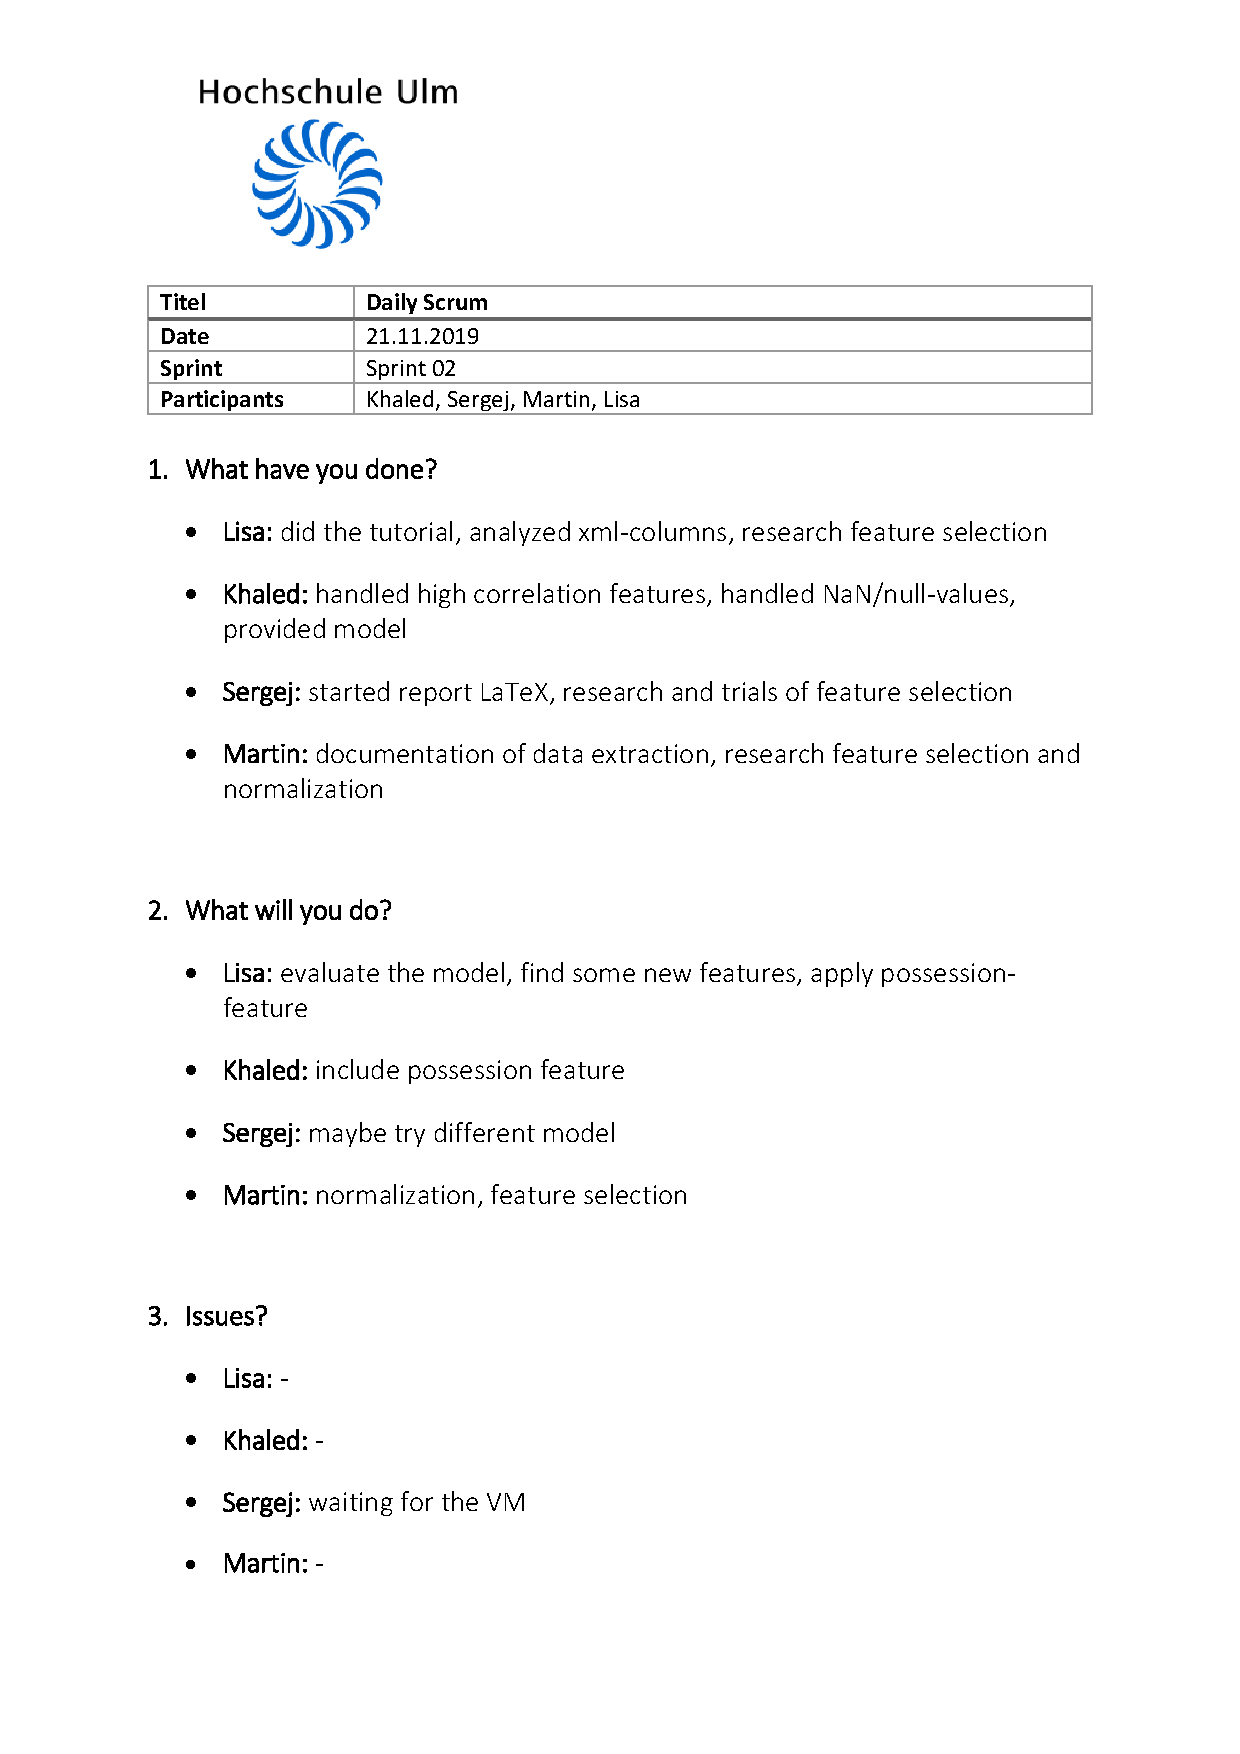
\includepdf[pages={1-2}]{pdf/Daily_Scrum_S02_3.pdf}
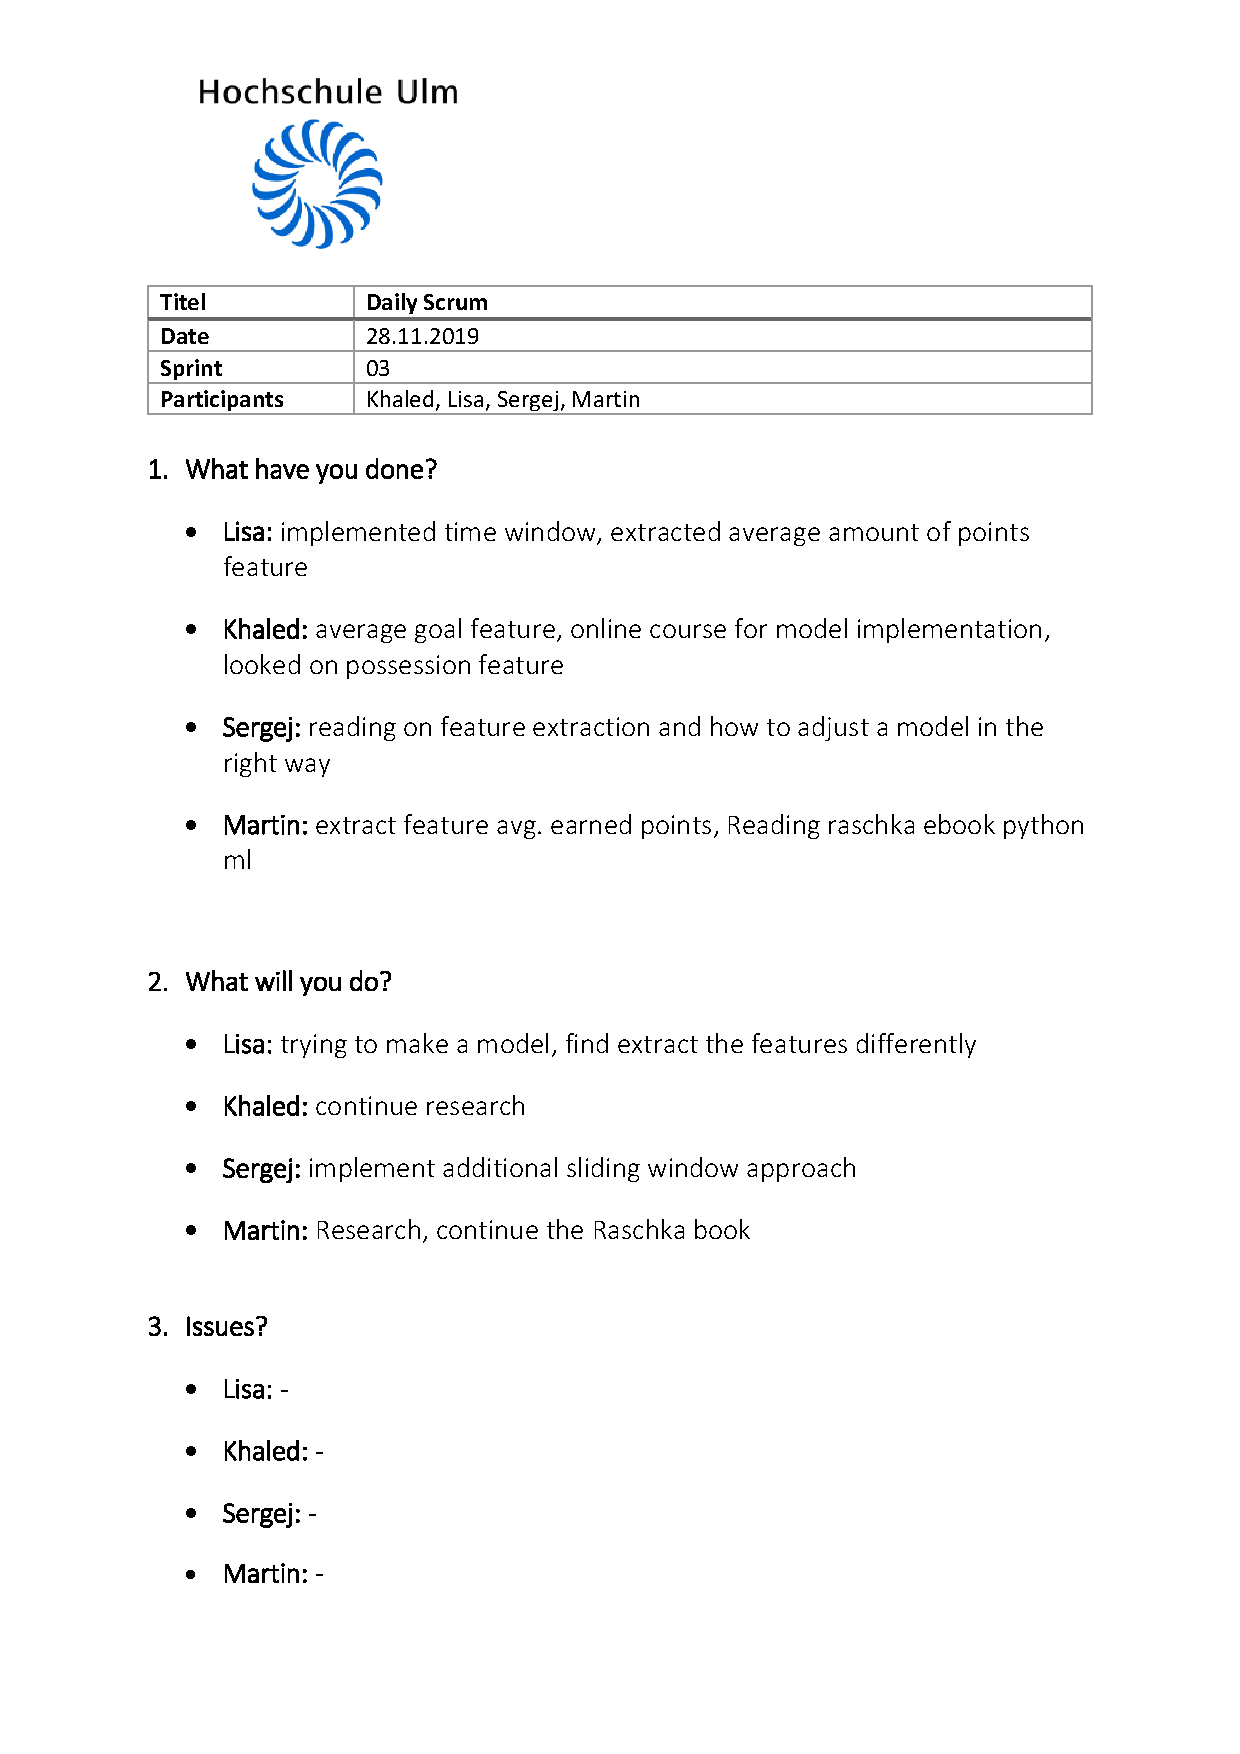
\includepdf[pages={1-2}]{pdf/Daily_Scrum_S03_1.pdf}
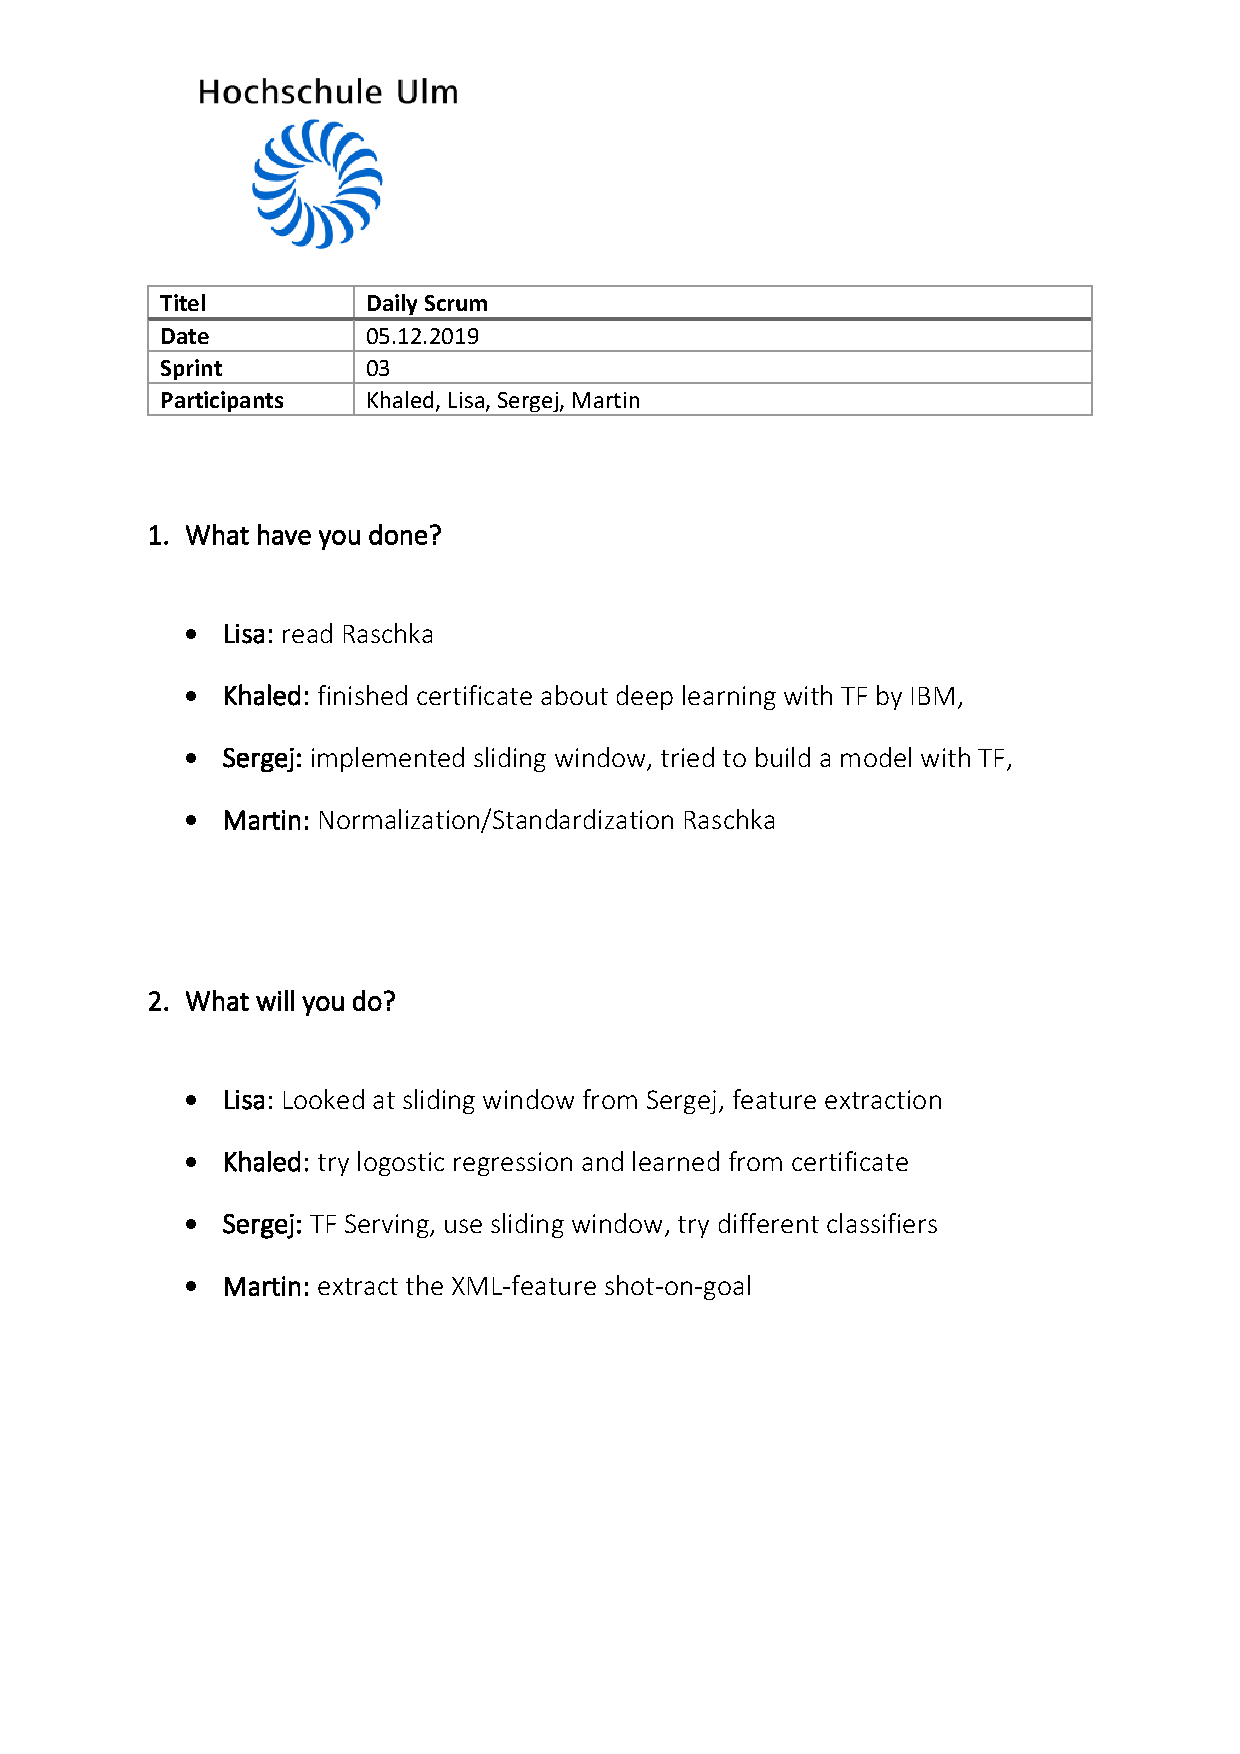
\includepdf[pages={1-2}]{pdf/Daily_Scrum_S03_2.pdf}
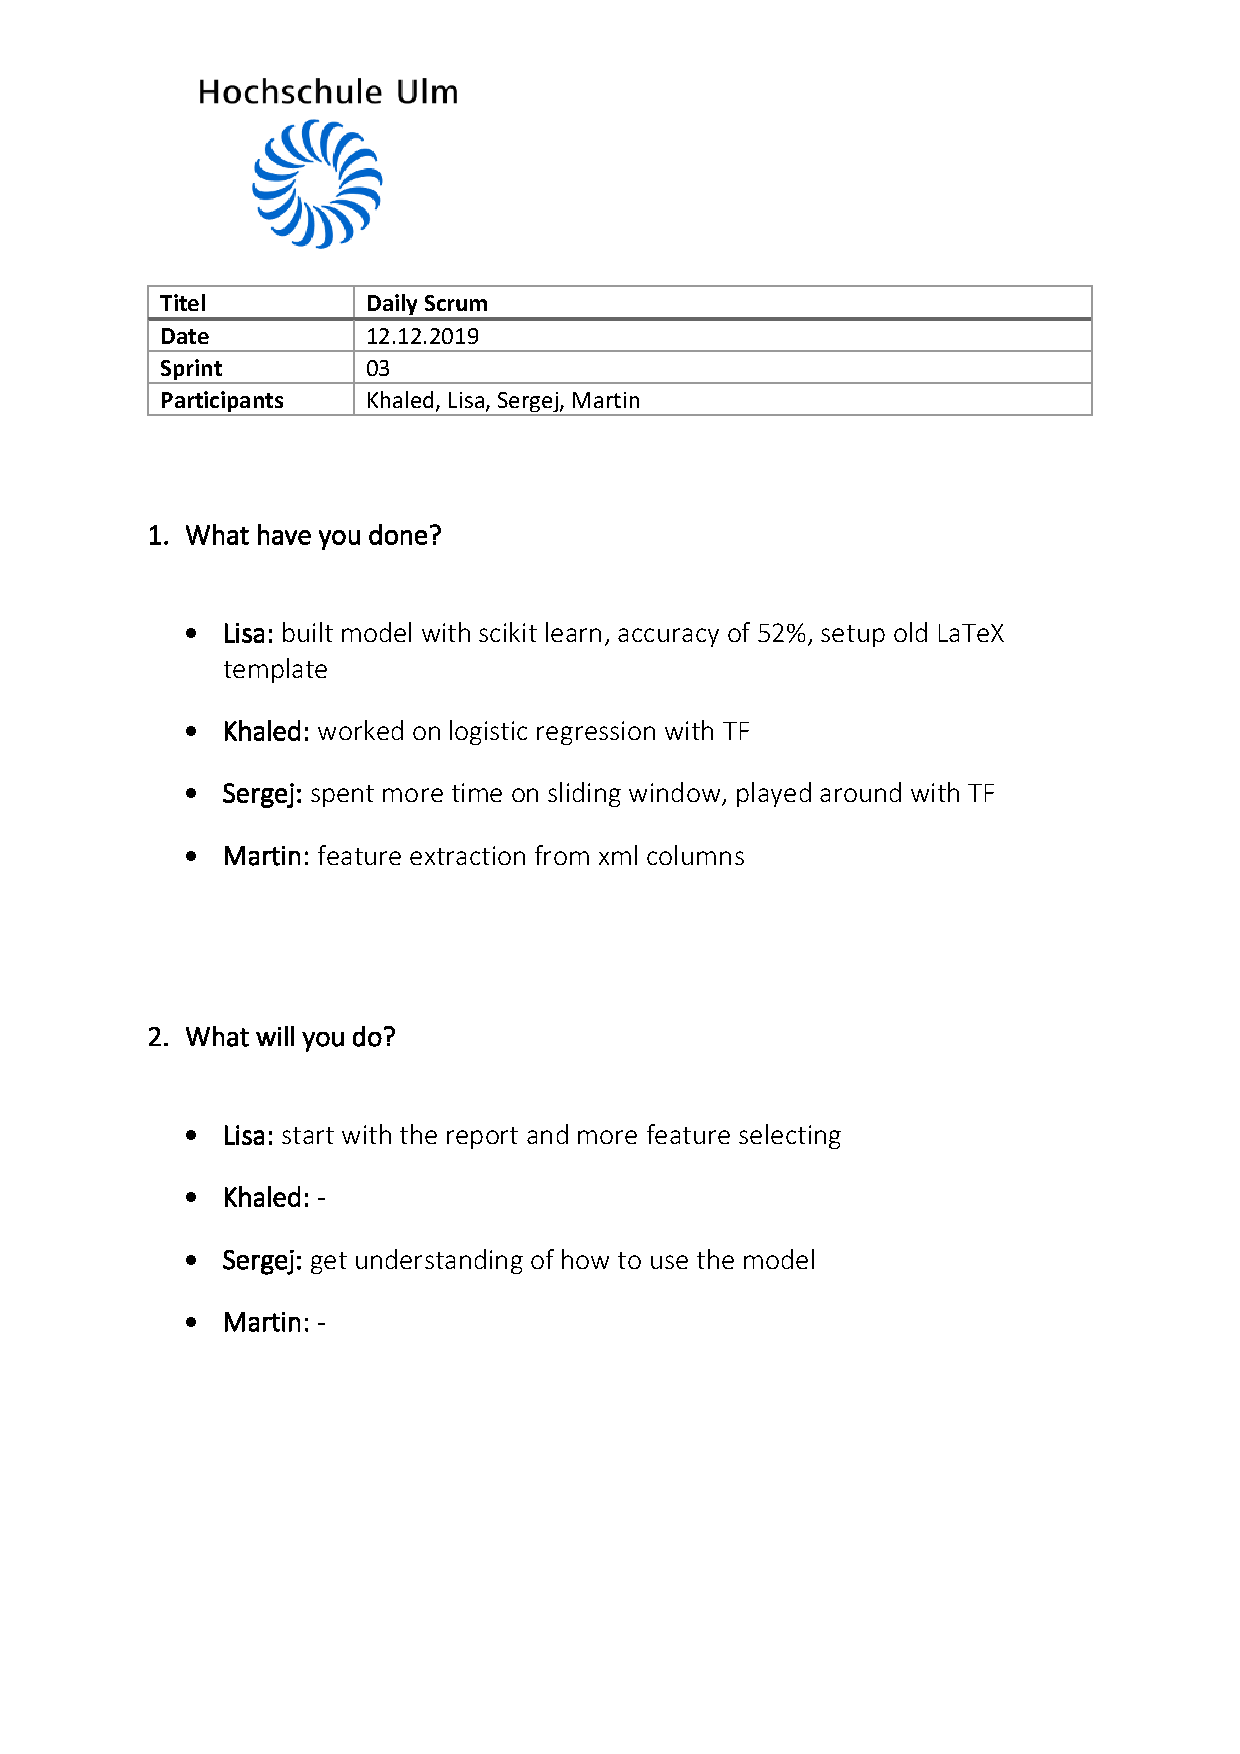
\includepdf[pages={1-2}]{pdf/Daily_Scrum_S03_3.pdf}
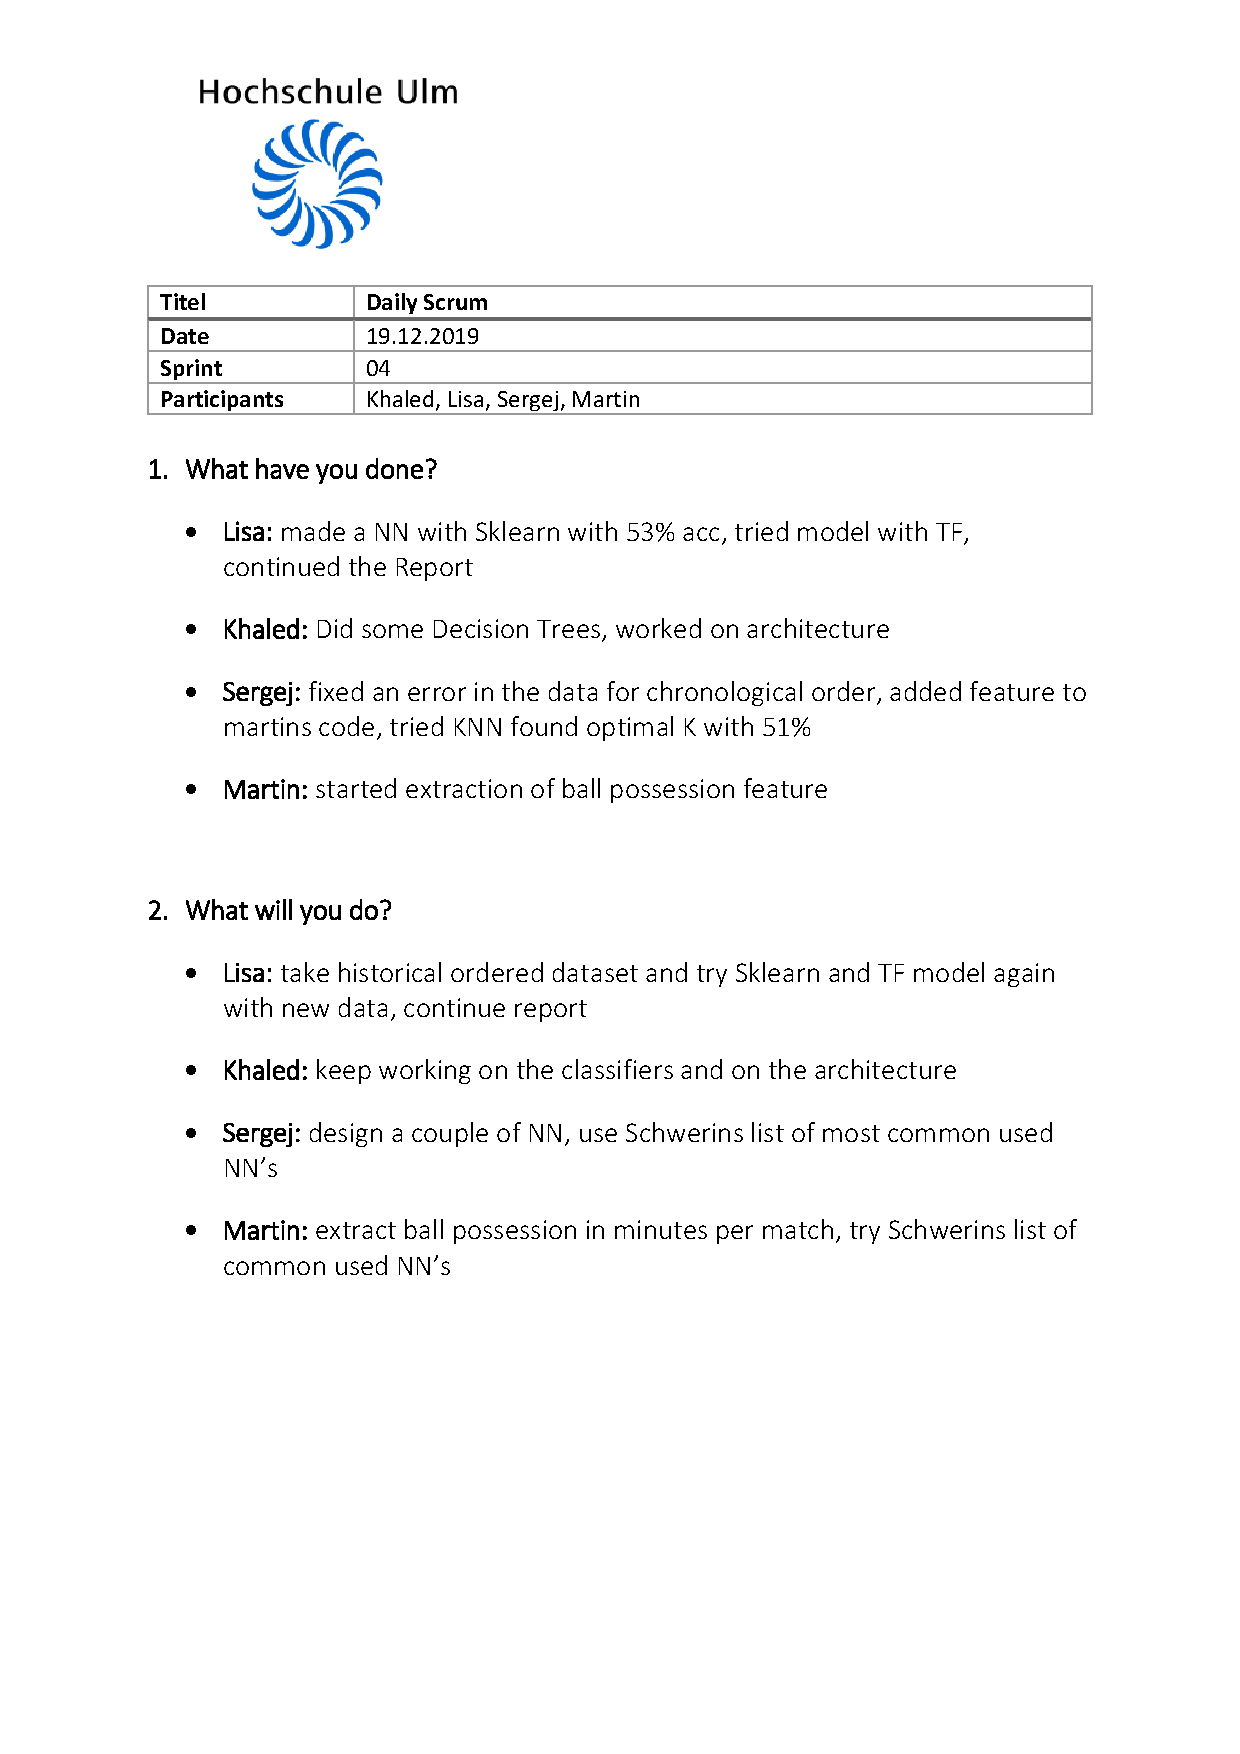
\includepdf[pages={1-2}]{pdf/Daily_Scrum_S04_1.pdf}
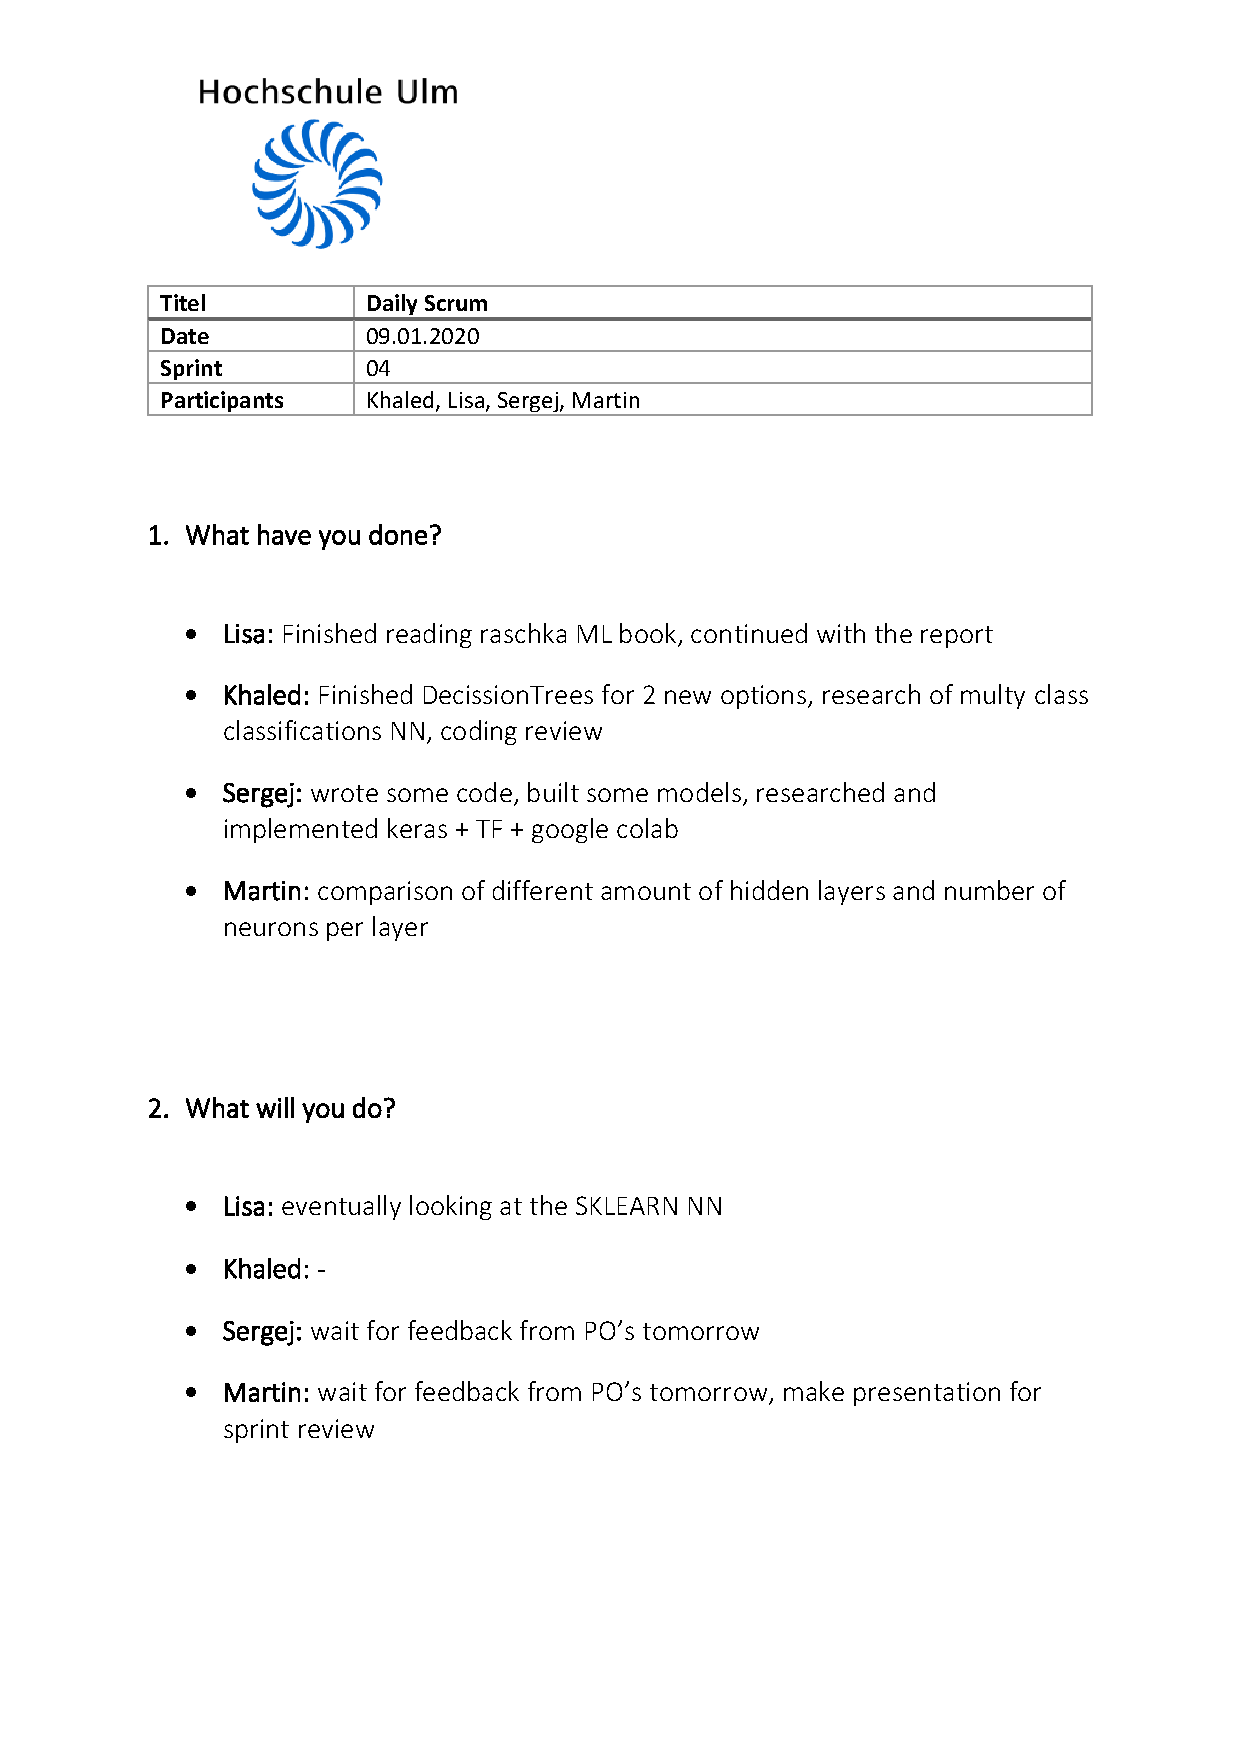
\includepdf[pages={1-2}]{pdf/Daily_Scrum_S04_2.pdf}

\newpage
\section{ Report of First Semester}
\label{section:appendix_c}
\newpage
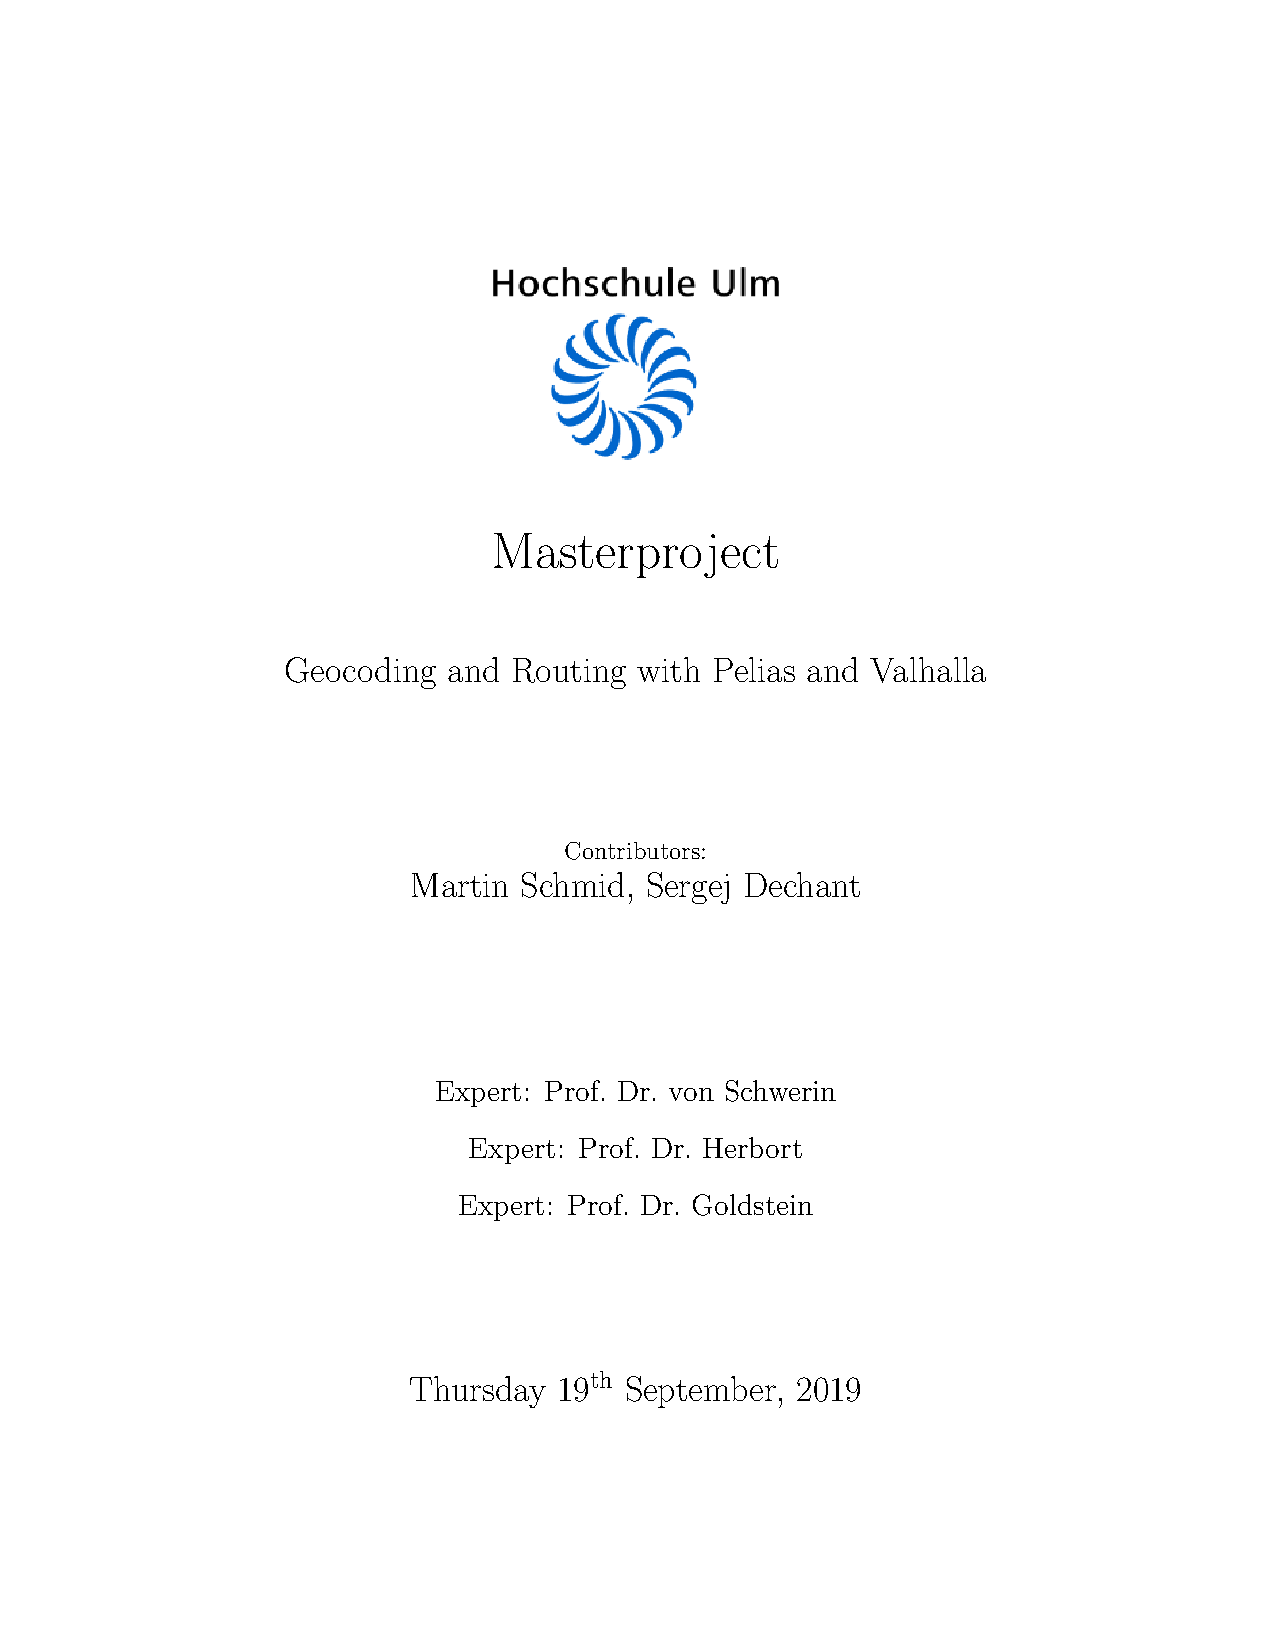
\includepdf[pages={1-30}]{pdf/ReportSemester1.pdf}

	
\end{document}
